\documentclass[10pt]{beamer}

\usetheme[progressbar=frametitle]{metropolis}
\usepackage{appendixnumberbeamer}

\usepackage{booktabs}
\usepackage[scale=2]{ccicons}

\usepackage{pgfplots}
\usepgfplotslibrary{dateplot}
\definecolor{customgrey}{RGB}{240,240,240} % Light grey
\definecolor{customorange}{RGB}{255,102,0} % Orange

\setbeamercolor{block title alerted}{fg=white,bg=customorange}
\setbeamercolor{block body alerted}{fg=black,bg=customgrey}
\setbeamerfont{block title alerted}{series=\bfseries}
\setbeamerfont{block body alerted}{}
\usepackage{xspace}
\newcommand{\themename}{\textbf{\textsc{metropolis}}\xspace}

\title{Pricing Agents and Algorithmic Collusion in Retail Oil Markets}
\subtitle{Case study from the Australian Market}

% \date{\today}
\date{}
\author{Lucia Sauer, Julian Romero \& Moritz Peist }
\institute{Barcelona School of Economics}
% \titlegraphic{\hfill\includegraphics[height=1.5cm]{logo.pdf}}

\begin{document}

\maketitle


\begin{frame}{Research question}
    \begin{alertblock}{Research question}
        \centering
        \textbf{Can LLMs replicate coordination behavior observed in real-world retail gasoline pricing?}
    \end{alertblock}
    %Can LLMs based-pricing agents coordinate around a focal point in a simulated retail gas industry? 
    \bigskip
    Motivation papers:
    \begin{enumerate}
        \item Algorithmic Collusion by LLMs (Fish et al., 2025)
        \item Learning to Coordinate: A Study in Retail Gasoline (Byrne \& Roos, 2019)
    \end{enumerate}
\end{frame}


\begin{frame}[fragile]{Algorithmic Collusion by LLMs}
%\textbf{Paper objective}: analyze AI delegation of economic decision-making task and economic outcomes.\\

    \begin{columns}
        % Left column: text
        \begin{column}{0.55\textwidth}
     \includegraphics[width=\linewidth]{slides_pricing_collusion/imgs/dupoly_experiment.png}
        \end{column}
    
        % Right column: image
        \begin{column}{0.55\textwidth}
        \textbf{Objective:} Analyze AI delegation of economic decision-making tasks and economic outcomes.
        
         Conduct experiments on LLM-based pricing agents and study if multiple firms price using LLMs can result in autonomous collusion? Yes!      
        \end{column}
    \end{columns}
P1: ``...your primary goal of maximizing profit...''

P2: ``...pricing lower than your competitor will typically lead
to more product sold...''

\end{frame}


\begin{frame}[fragile]{Algorithmic Collusion by LLMs}
We replicate this paper using Open Source Models, where \textbf{Mistral LLMs show agentic pricing capabilities and collusive behavior}.
\begin{columns}
    % Left column: text
    \begin{column}{0.55\textwidth}
 \includegraphics[width=\linewidth]{imgs/dupoly_experiment.png}
  \caption{\textbf{Original} - ChatGPT-4}
    \end{column}

    % Right column: image
    \begin{column}{0.55\textwidth}
           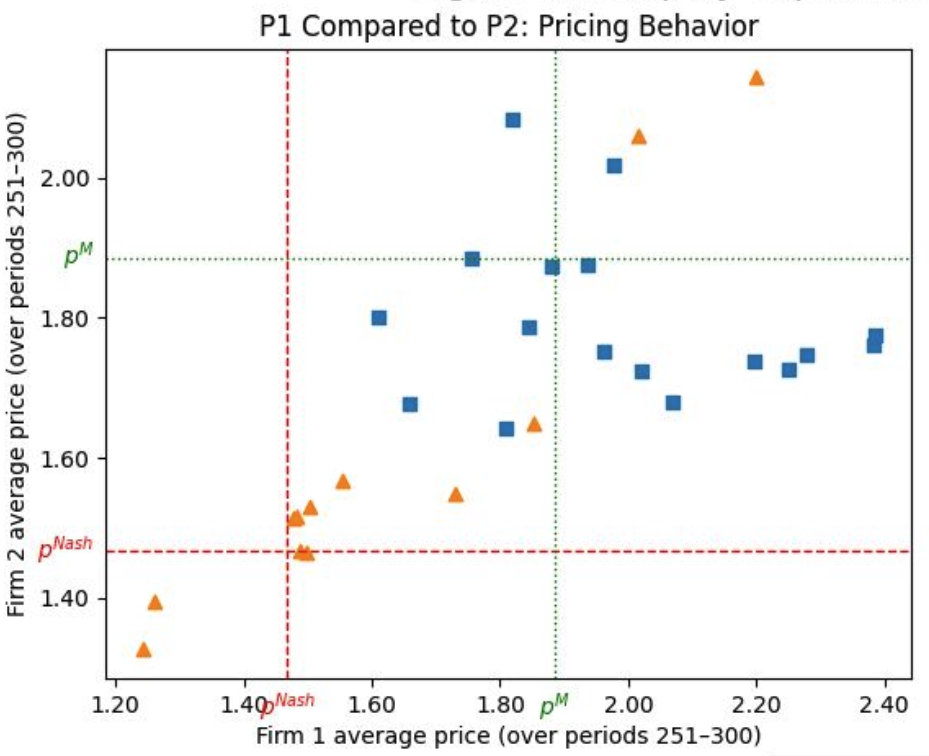
\includegraphics[width=\linewidth]{imgs/duopoly_experiment_replication.png}
           \caption{\textbf{Replication} - MistralAI}
    \end{column}
\end{columns}


\end{frame}





\subsection{}


\begin{frame}[fragile]{Learning to coordinate}
They analyze tacit collusion in Australian fuel market. By law, retailers are mandated to notify publicly their next-day prices and keep them fixed for 24 hs.

    \begin{columns}
        % Left column: text
        \begin{column}{0.55\textwidth}
            \begin{itemize}
                \item Repeated Game, with Homogenous Price, Symmetrics Marginal Cost (TGP) and perfect information.
                \item \textbf{Price leadership} BP started increasing prices and this gives it the informational role of signaling a price intention to the other firms that coordinate, creating tacit collusion.
                \item \textbf{Market shares constants through time.}
            \end{itemize}
        \end{column}
    
        % Right column: image
        \begin{column}{0.55\textwidth}
            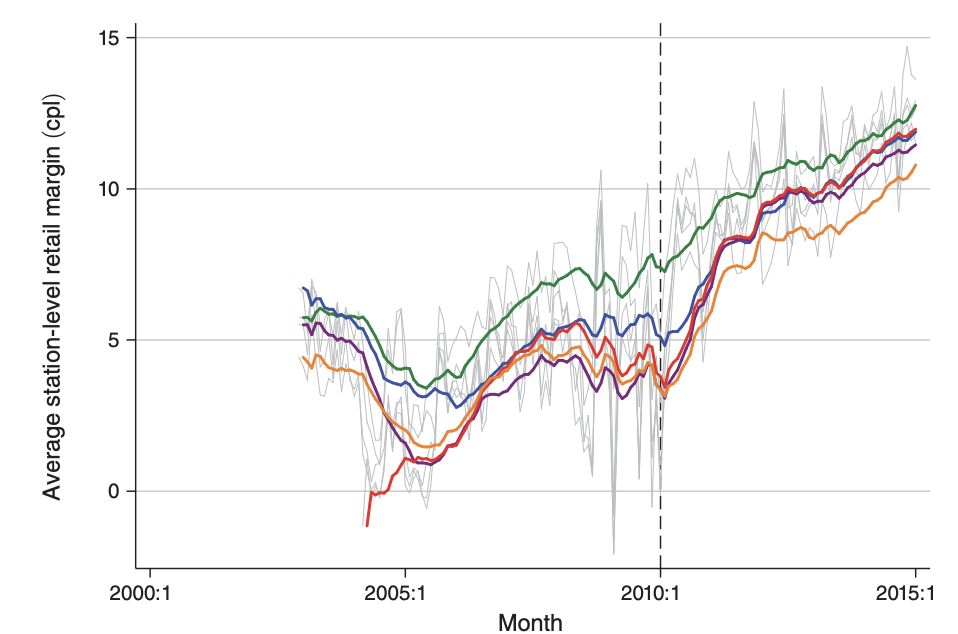
\includegraphics[width=\linewidth]{slides_pricing_collusion/imgs/avg_margins_by_firm.png}
            
        \end{column}
    \end{columns}

\end{frame}

\subsection{}

\begin{frame}[fragile]{Our Implementation}
\begin{figure}
    \centering
    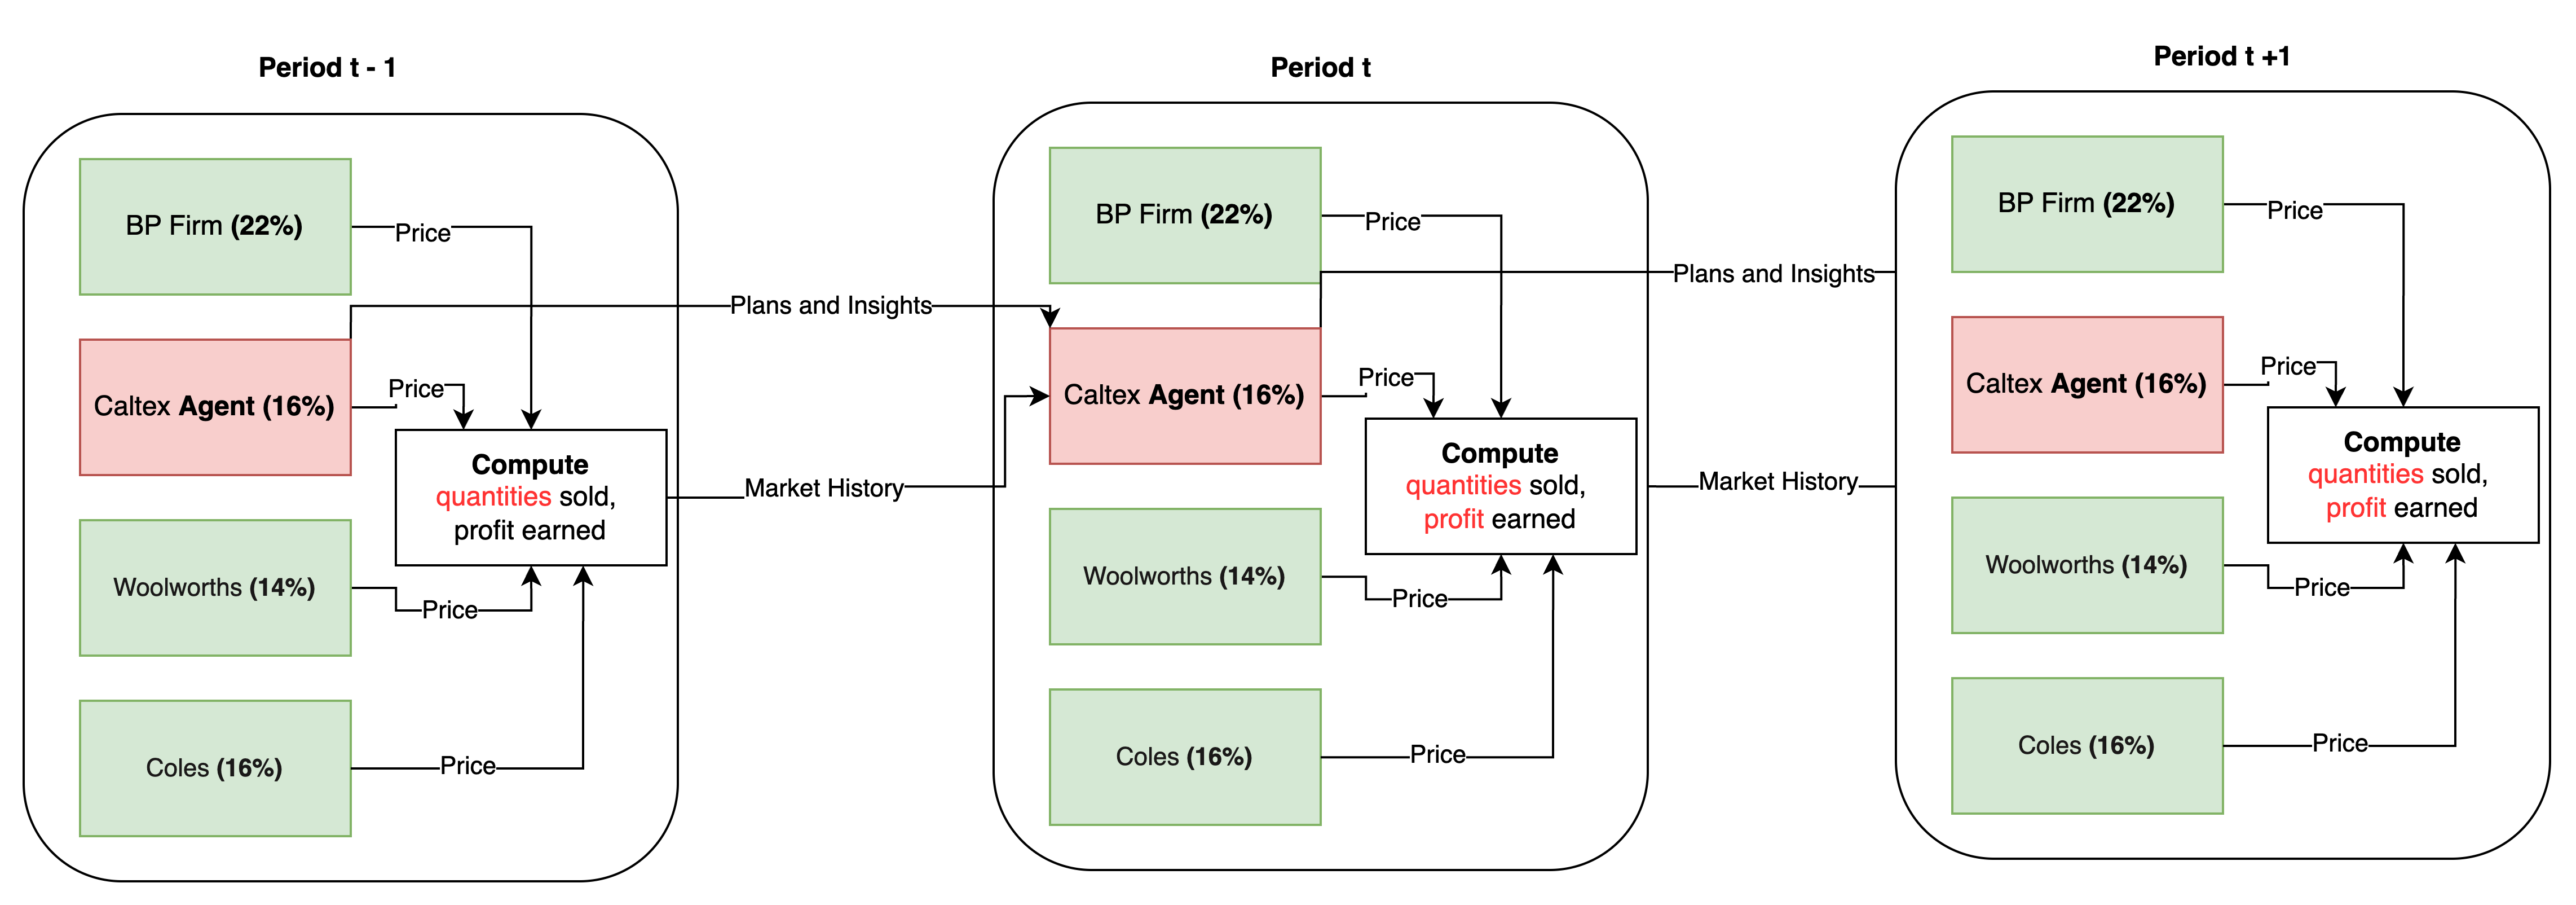
\includegraphics[width=1.5\linewidth]{slides_pricing_collusion/imgs/diagram.png}
    \caption{}
    \label{fig:enter-label}
\end{figure}
  
\end{frame}

\begin{frame}[fragile]{Demand function}
Currently, we are investigating how to make the agent receive an answer from the environment:
\begin{itemize}
    \item Calvano (2020) Demand Function
    $$
q_i = \beta \cdot \frac{e^{\frac{a_i - p_i/\alpha}{\mu}}}{\sum_{j=1}^{n} e^{\frac{a_j - p_j/\alpha}{\mu}} + e^{\frac{a_0}{\mu}}}
$$
\begin{itemize}
    \item $a_1, a_2, \ldots, a_n$: product-specific attributes (differentiation), with $a_0$: baseline demand intercept.
    \item $\alpha=1, \beta=100$: scaling parameters. $\alpha$ affects currency unit, $\beta$ quantity scaling factor.
    \item $a_0 = 0$, $\mu = 0.25$, all from Calvano et al. (2020b).
\end{itemize}
    \item Focus on markup, taking advantage of the real market structure
    \begin{itemize}
        \item ⁠Inelastic demand (people need gas regardless)
        \item Sticky market shares due to location/convenience
        \item Competition primarily on margins, not volume
    \end{itemize}
\end{itemize}
  
\end{frame}



%\appendix

%\begin{frame}[fragile]{Backup slides}
% -
%\end{frame}

%\begin{frame}[allowframebreaks]{References}

%  \bibliography{demo}
%  \bibliographystyle{abbrv}

%\end{frame}

\end{document}
